\chapter{Konzeption und Implementierung}
\section{Anwendungsfunktionalität}
%TODO
\section{Konzeptentwicklung}
	In diesem Abschnitt werden grundlegende Aspekte der Softwarearchitektur vom GuttenBase Plugin vorgestellt. Diese werden basierend auf der Empfehlung im IEEE-Standard IEEE STD 1471-2000 erstellt.\\
	Die Architektur wird aus zwei Sichten Sichten (Views) betrachtet. Eine Sicht repräsentiert dabei das Softwaresystem aus der Perspektive einer verwandten Menge von Aspekten. Jede Sicht stellt spezifische Informationen bereit.\\
	Es is außerdem zu beachten, dass sich die Architektur auf die Ergebnisse der funktionalen Anforderungsanalyse sowie auf die Architektur der Zielplattform (IntelliJ Plattform) bezieht.
	Im Folgenden werden die einzelnen Sichten genauer vorgestellt.
	%TODO zitieren




	\subsection{Konzeptionelle Sicht}
	Im Folgenden wird die Konzeptionelle Sicht des Systems vorgestellt. Hier wird das System noch unabhängig von den Implementierungsentscheidungen betrachtet. \\
	Die konzeptionelle Sicht wird als Komponentendiagramm in der Abbildung \ref{img:component-diagram} dargestellt. 
	\begin{figure}[H]
		\centering
		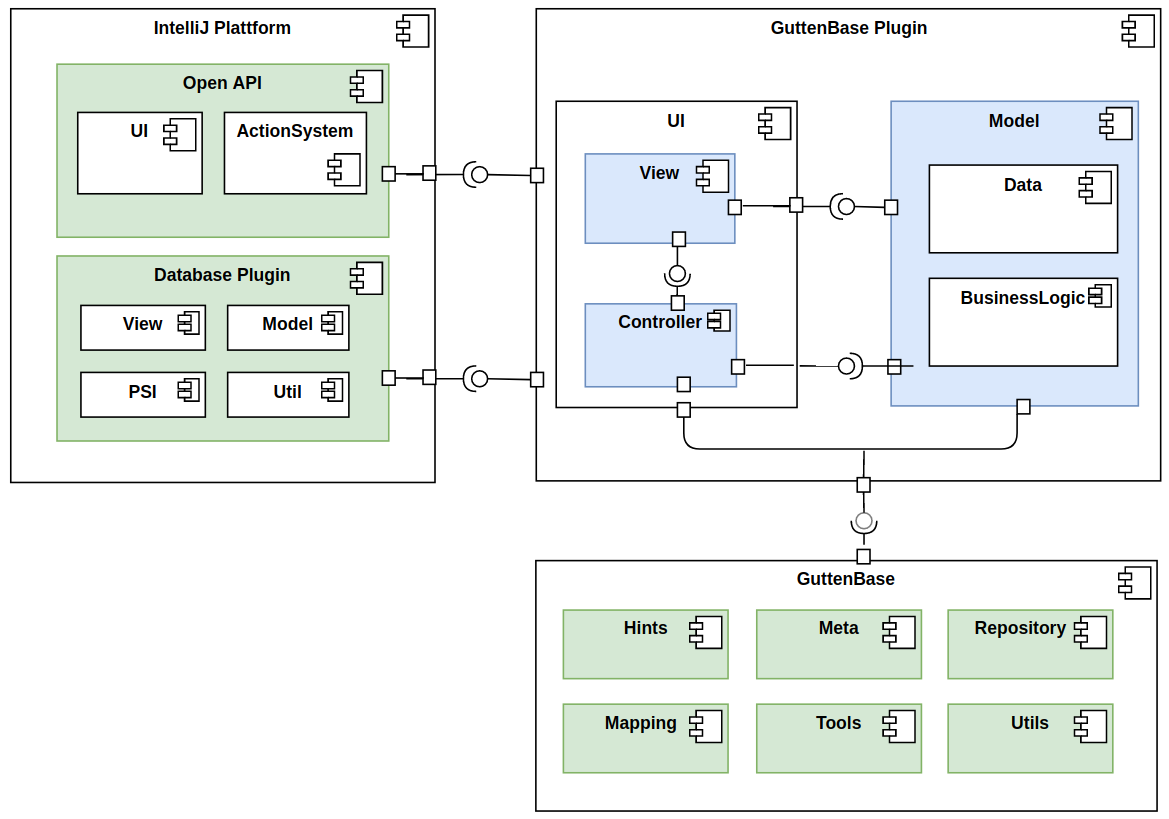
\includegraphics[width=\textwidth]{images/sichten/component-diagram}
		\caption{Komponentendiagramm für die konzeptionelle Sicht}
		\label{img:component-diagram}
	\end{figure}
	Das Komponentendiagramm besteht aus der GuttenBase Plugin Komponente, welche das zu entwickelnde System darstellt, der IntelliJ Plattform Komponente und der GutteBase Komponente. Es werden nur Komponenten veranschaulicht, die von unserem System benötigt sind. Diese werden im Folgenden genauer beschrieben.
	
	
	\subsubsection{GuttenBase Plugin}
	Das GuttenBase Plugin wird nach dem MVC-Arcchitekturstil konzipiert und besteht aus folgenden Komponenten:
	
	\paragraph*{Model}
	Das Modell enthällt Daten, die von der View Komponente dargestellt werden. Hier liegt außerdem die Geschäftslogik(\textbf{BusinessLogik}), welche für die Änderung der Daten zuständig ist.
	
	\paragraph*{View}
	Die View Komponente ist für die Darstellung der Daten für den Benutzer verantwortlich. Hier werden alle UI-abhängigen Aspekte wie Layout, Schriftart usw. behandelt.\\
	
	\paragraph*{Controller}
	Die Controlle Komponente ist für die Interaktion mit dem Benutzer verantwortlich. Sie wird von der View Komponente über Benutzerinteraktionen informiert und wertet sie aus. Anschließend können Änderungen an den Daten der Model Komponente sowie Anpassungen an der View Komponente angonommen werden.
	
	\subsubsection{IntelliJ Plattform}
	Wie in der Abbildung \ref{img:component-diagram} zu sehen ist, interagiert das GuttenBase Plugin mit mehreren Komponenten der IntelliJ Plattform. 
	Es wurden dabei nur die verwendeten Komponenten dargestellt. Diese sind in zwei Komponenten beinhaltet:
	
	\paragraph*{Open API}
	Die IntelliJ Open API beinhaltet viele Komponenten, die auch von der IntelliJ IDEA Community Edition verwendet werden und für Plugin-Entwickler zur Verfügung stehen. Es können z. B. UI-Komponenten aus der Komponente \textbf{UI} für die Implementierung des Plugins benutzt werden. Außerdem wird \textbf{ActionSystem} Komponente benötigt, um bestimmte Aktionen, wie das Starten des Plugins, auszulösen.
	\paragraph*{Database Plugin}
	Da das GuttenBase Plugin viel mit den Datenbanken umgeht, die in IntelliJ konfiguriert wurden, ist eine Interaktion mit dem Database Plugin sehr sinnvoll. Dazu bieten sich viele Komponenten für unterschiedliche Zwecke. Die für das GuttenBase Plugin benötigten Komponenten sind die \textbf{Model} Komponente (um evt. eine Datenbank Konfiguration zu bekommen), die \textbf{PSI} Komponente (um die Elemente der Datenbank zu bekommen), die \textbf{Util} Komponente (um ein Datenbank-Schema zu bekommen) und die \textbf{View} Komponente (um aus der Übersicht des Database  Plugins Datenbank-Inhalte zu bekommen).
	
	
	%\subsubsection{GuttenBase} 
	%TODO
	
	
	
	
	\subsection{Modulsicht}
	Die Modulsicht zeigt die Struktur des GutenBase Plugins in Form von Modulen und deren Beziehungen zueinander. Hierbei werden die Komponenten und Konnektoren der konzeptionellen Sicht auf Module, Schichten und Subsysteme abgebildet. Diese werden in Paket- und Klassendiagramme verfeinert.
	Zur Wahrung der Übersichtlichkeit wird die Modulsicht nach den unterschiedlichen Übersichten unterteilt. Es gibt insgesamt vier Übersichten, die das gesammte System abdecken. Pro Übersicht werden nur Klassen bzw. Methoden beschrieben, die entsprechenden Anwendungsfälle realisieren.
	
	\subsubsection{Modulsicht der Übersicht der Konfogurationsschritte}
	Die Modulsicht der Abbildung \ref{img:modulsicht-gbactions} beschreibt alle beteiligten Klassen, die beim Erstellt und Verwalten der Konfigurationsschritte eingesetzt sind. Diese werden entsprechend der Konzeptionellen Sicht aufgeteilt, nämlich in den View, Model und Controller Paketen.\\
	%-View Klassen sind für die UI - Swing KOmponenten.
	%- Controlle hat folgende Aufgaben: 
	%- UI Komponenten erstellen, 
	%- Aktionen erstellen: die GBActionView informiert controller über Benutzer Eingabe -> jenachdem welchen ActionTyp selektiert wurde, wird die entsprechende DumbAwareAction ausgeführt, damit die entsprechende Dialoge für das Erstellen der Action angezeigt wird (renameView + changeType))
	%- editieren und speichern: nach dem Klick auf Save wird die Save Methode des Controller aufgerufen, sodass alle hinzugefügten Konfigurationsschritte mithilfe der GsonHelper konvertiert und gespeichert werden.
	%- actionen darstellen, 
	%- Übersicht schließen: Nach dem Klick auf cancel wird die Übersicht geschlossen.
	\begin{figure}[H]
		\centering
		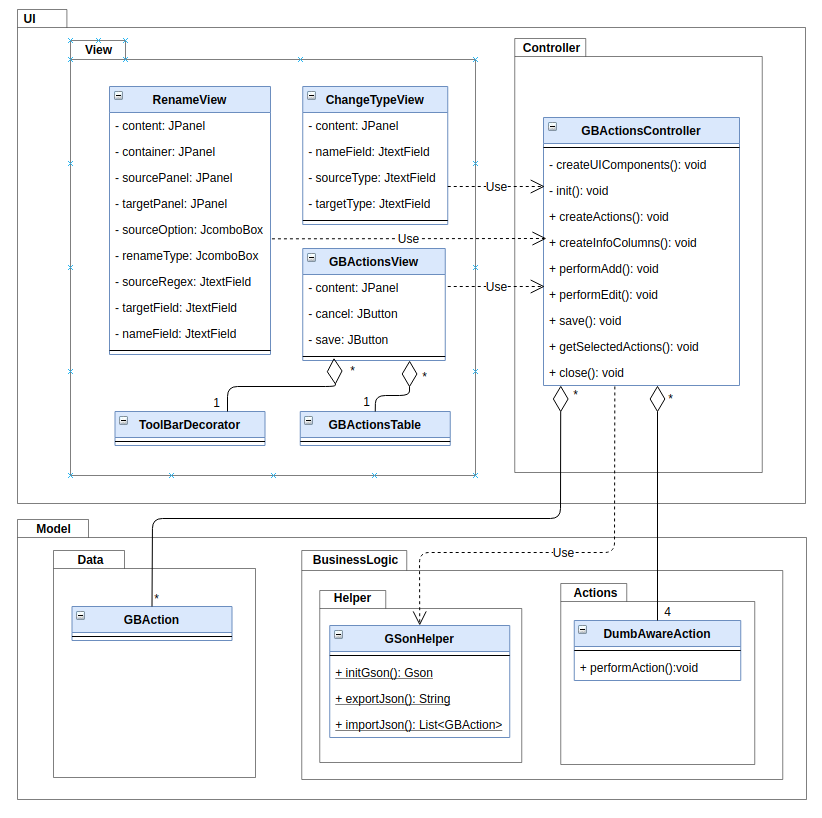
\includegraphics[width=\textwidth]{images/sichten/modulsicht-gbactions}
		\caption{Modulsicht der Übersicht der Konfogurationsschritte}
		\label{img:modulsicht-gbactions}
	\end{figure}
	In dem View Paket werden alle Klassen dargestellt, die für die Darstellung der Konfigurationsschritte zuständig sind. Diese basieren auf unterschiedliche Swing Komponenten. Die Klasse GBActionsView repräsentiert dabei die Hauptübersicht der Konfigurationsschritte und beeinhaltet die GBActionsTable Klasse, welche die Auflistung der Konfigurationsschritte übernimmt. Außerdem wird die ToolbarDecorator Klasse für die Darstellung der möglichen Aktionen benötigt. \\
	Das Controller Paket enthält hierbei die GBActionsController Klasse. Diese hat folgende Aufgaben:
	\begin{itemize}
		\item UI-Komponenten vor dem Anzeigen vorbereiten, indem Daten aus dem Paket Model erzeugt bzw. geladen werden.
		\item Konfigurationsschritte erstellen. Dies passiert nach der Benuzter einen bestimmten Konfigurationsschritt hinzufügen möchte und diesen in der GBActionsView übersicht selektiert. Zunächst wird die entsprechende DumbAwareAction Klasse aufgerufen, um die entsprechende Aktion durchzuführen. Die DumbAwareAction Klasse ist im Paket BusinessLogic zu finden und könnte z. B. für das Anzeigen der Übersicht für das Erstellen des Umbenennen- oder Datentyp-Ändern-Konfigurationsschritt verwendet werden. Diese werden durch die RenameView und ChangeTypeView Klassen realisiert. Analog dazu erfolg das Editieren der Konfigurationsschritte.
		\item Konfigurationsschritte speichern, indem die hinzugefügte Konfigurationsschritte in JSON konvertiert und dann exportiert werden. Dafür ist die GsonHelper Klasse des BusinessLogic Pakets zuständig.
	\end{itemize}
	
	
	
	\subsubsection{Modulsicht der allgemeinen Übersicht}
	Diese Modulsicht zeigt die beteiligten Klassen, die beim Verbinden der zu migrierenden Datenbanken genutzt werden. Diese wird in der Abblidung \ref{img:modulsicht-general} dargestellt. 
	\begin{figure}[H]
		\centering
		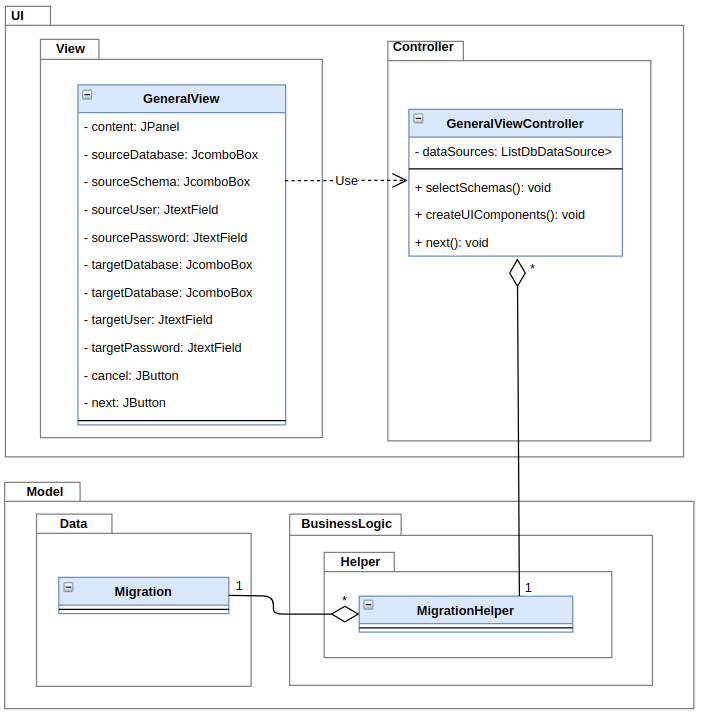
\includegraphics[width=0.7\textwidth]{images/sichten/modulsicht-general}
		\caption{Modulsicht der allgemeinen Übersicht}
		\label{img:modulsicht-general}
	\end{figure}
	Die GeneralView Klasse ist für die Interaktion mit dem Benutzer verantwortlich und enthält alle Eingabefelder und Texte. Die GeneralViewController Klasse ist für das Laden der Datenbankelemente zuständig. Klickt der Benutzer auf das \glq Next\grqq Button, werden alle Eingaben über die MigrationHelper Klasse des Pakets BusinessLogic übergeben. Diese Informationen werden dann in der Migration Klasse des Model Pakets gespeichert.
	
	
	\subsubsection{Modulsicht der Konfigurationsübersicht}
	Die Modulsicht in der Abbildung \ref{img:modulsicht-overview} zeigt die für die Konfigurationsübersicht relevanten Klassen.
	\begin{figure}[H]
		\centering
		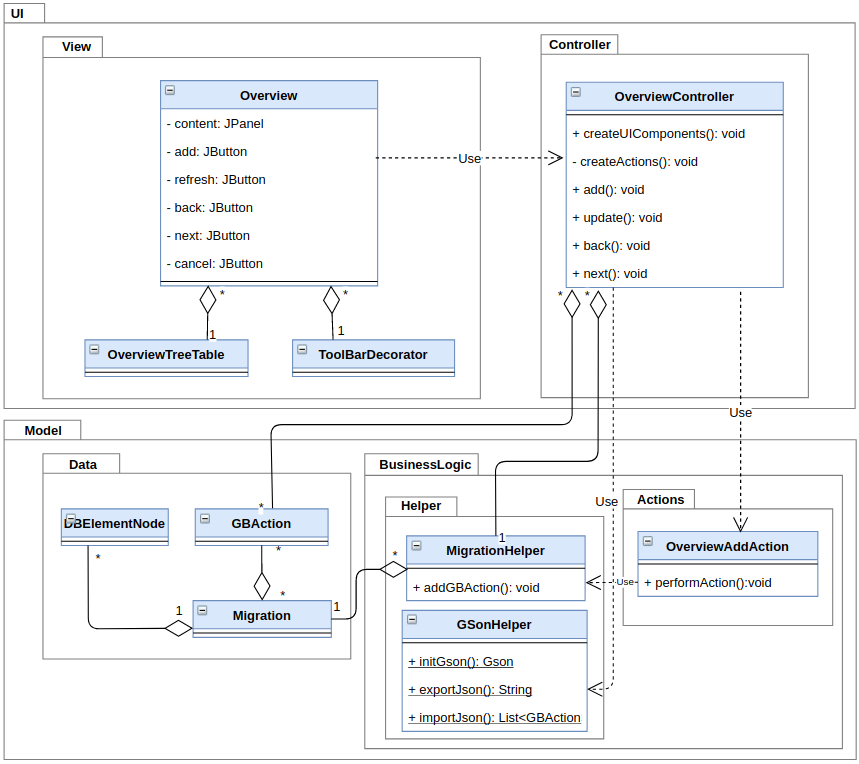
\includegraphics[width=\textwidth]{images/sichten/modulsicht-overview}
		\caption{Modulsicht der Konfigurationsübersicht}
		\label{img:modulsicht-overview}
	\end{figure}
	In der Konfigurationsübersicht (Overview) enthält die OverviewTreeTable Klasse, welche alle Quell-Datenbankelemente auflistet und die ToolbarDecorator Klasse, die gespeicherten Konfigurationsschritte anzeigt. Außerdem stehen einige Buttons für die Benutzerinteraktion zur Verfügung. \\
	Wie bei den vorherigen Modulsichten, stellt die OverviewController Klasse Methoden für folgende Zwecke bereit:
	\begin{itemize}
		\item Das Laden der Datenbankelemente: Hierbei werden die gespeicherten Konfigurationsschritte mithilfe der GsonHelper Klasse importiert und die Datenbankelement (DBElementNode) aus der Quell-Datenbank erstellt.
		\item das Anzeigen der Konfigurationsschritte: Konfigurationsschritte werden nach Kompatibiltät mit den selektierten Datenbankelementen behandelt. Ist ein Konfigurationsschritt mit einem Datenbankelent geeignet, wird dieser klickbar angezeigt, außerdem wird stattdessen ein ausgegrautes Button dargestellt.
		\item Hinzufügen von Konfigurationsschritten: Wenn der Benutzer ein Datenbankelement selektiert und dann einen entsprechenden Konfigurationsschritt hinzufügt, wird die OverviewAddAction Aktion von dem BusinessLogic Paket ausgelöst. Dabei wird der entsprechende Konfigurationsschritt durch die MigrationHelper Klasse zur Migration hinzugefügt.
	\end{itemize}
	
	
	
	\subsubsection{Modulsicht der Ergebnisübersicht}
	Die Modulsicht der Abbildung \ref{img:modulsicht-resul} stellt die für die Ergebnisübersicht (ResultView) zuständigen Klassen. Außerdem wird die Fortschritt Übersicht (ProgressView) miteingebunden, da diese vom selben Controller verwaltet wird.
	\begin{figure}[H]
		\centering
		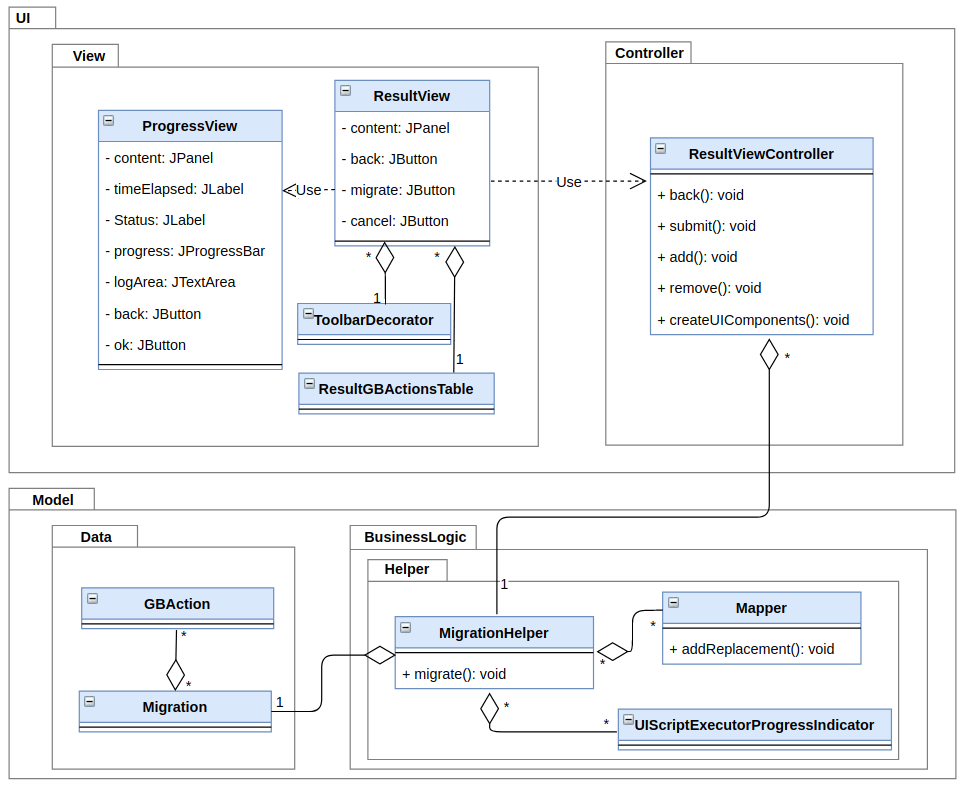
\includegraphics[width=\textwidth]{images/sichten/modulsicht-result}
		\caption{Modulsicht der Ergebnisübersicht}
		\label{img:modulsicht-resul}
	\end{figure}
	Ähnlich wie bei den anderen Übersichten, enthältt die ResultView Klasse eine Tabelle (ResultGBActionsTable), die alle hinzugefügten Konfigurationsschritte enthält und ein ToolbarDecorator, wo die Aktionen zum Löschen und Hinzufügen angezeigt werden. \\
	Auf der anderen Seite stellt die ResultViewController Klasse Methoden für das Löschen und das Hinzufügen von Konfigurationsschritte sowie für das Starten des Migrationsprozesses bereit. Diese werden im Folgenden genauer erklärt:
	\begin{itemize}
		\item Hinzufügen: Wenn der Benutzer noch mehr Konfigurationsschritte zur Migration hinzufügen möchte, wird die aktuelle Übersicht zur Übersicht der Konfigurationsschritte (Overview) umgeleitet.
		\item Löschen: Wie das Hinzufügen, erfolgt das Löschen von Konfigurationsschritte (die schon zur Migration hinzugefügt wurden) durch die Entfernung von dem ausgewählten Konfigurationsschritt (GBAction) aus der Migration Klasse. 
		\item Migration starten: Nach dem Klick auf das \glqq Migrate\grqq Button, wird der Migrationsprozess gestartet. Dieser erfolgt durch die MigrationHelper Klasse. Dabei wird das Connector Repository der GuttenBase Bibliothek entsprechend der Konfigurationsschritte konfiguriert (siehe \ref{section:grundlagen:gb}) und anschließend das Kopieren durch das DefaultTableCopyTool gestartet. \\
		Parallel dazu wird die Fortschritt Übersicht (ProgressView) angezeigt, um Informationen über den laufenden Prozess zu sehen. Dies ist durch die UIScriptExecutorProgressIndicator Klasse ermöglicht.
		
		%	- add connectors, cfg abgeschlossen -> Copy 
		%	- parallel dazu: Fortschritt übersicht anzeigen: Logginging: Logging Hin.
	\end{itemize}


\section{Technologieauswahl}
	
	\section{Umsetzungsform}
	Um eine optimale Nutzung des GuttenBase Plugins zu erzielen, soll auf die Umsetzungsform geachtet werden.\\
	Das zu entwickelnde Tool kann z. B. als eine Desktop Applikation, Web Applikation oder als Plugin einer anderen Anwendung realisiert werden.\\
	In der Tabelle \ref{table:tool-options} werden einige Vor- und Nachteie jeder Alternative erläutert. \\
	Alle drei Alternativen haben Pros und Contras allerdings ist die schnellere Erreichung von vielen Nutzern sowie die Einfache Installation bei der IDE Plugin Entwicklung entscheidend. 
	\begin{table}
		\centering
		\begin{tabular}{ |p{3cm}|p{6cm}|p{6cm}| }
			\hline
			\textbf{Alternative} & \textbf{Vorteile} &  \textbf{Nachteile}  \\
			Desktop App & 
			\begin{itemize}
				\item Offline immer verfügbar
				\item Volle Kontrolle über die Anwendung und die enthaltenen Daten.
				\item Bessere Leistung, da kein Browser als Zwischenschicht existiert.
			\end{itemize}& 
			\begin{itemize}
				\item Platformabhängig
				\item Hohe Entwicklungskosten
				\item Installation ist notwendig
			\end{itemize} \\
			\hline
			Web App &
			
			\begin{itemize}
				\item Installation oder manuelle Updates sind nicht notwändig. 
				\item geringere Entwicklung- und Wartungskosen, da die Anwendung unabhängig von lokalen Endgeräten ist.
			\end{itemize} &
			
			\begin{itemize}
				\item Offline meistens nicht verfügbar.
				\item Geringere Leistung.
			\end{itemize} \\
			\hline
			IDE Plugin Entwicklung &
			
			\begin{itemize}
				\item Für IntelliJ Benutzer ist das einfach und intuitiv zu benutzen.
				\item Manche Komponenten bzw. Funktionalitäten der zu erweiternden IDE können wiederverwwendet werden, was die Entwicklungsdauer verkürzt.
				\item Intuitive Nutzung sowie eine einheitliche Benutzeroberfläche wie die benutzte IDE.
			\end{itemize} &
			
			\begin{itemize}
				\item Die Flexibilität beim Entwickeln ist durch die limitierte Erweiterbarkeit der IDE eingeschränkt.
			\end{itemize} \\
			\hline
			
		\end{tabular}
		\caption{Umsetzungsmöglichkeiten}
		\label{table:tool-options}
	\end{table}
	
	Zunächst soll für eine konkrete IDE entschieden werden. Um diese auszuwählen, muss auf die Anzahl der Nutzer, die Verfügbarkeit der Dokumentation für Plugin Entwicklung sowie die Unterstützung von Datenbanken geachtet werden.\\
	Einer der bekanntesten Methoden, um die genaue Beliebtheit einer Programmiersprache bzw. eine IDE herauszufinden, ist der PYPL-Index. Er basiert auf Rohdaten aus Google Trends. PYPL enthält den TOP-IDE-Index, welches alanysiert, wie oft IDEs bei Google durchgesucht werden. Die Suchanfragen spiegeln zwar nicht unbedingt die Beliebtheit der IDEs. Allerdings hilft einen solchen Index enorm bei der Wahl einer Entwicklungsumgebung.
	Bei dieser Analyse sind die drei bekanntesten und für unseren Fall relevanten Entwicklungsumgebungen Visual Studio (erster Platz), Ecllipse (zweiter Platz) und IntelliJ (sechster Platz). Außerdem hat sich der Index von IntelliJ IDE am stärksten erhöht (siehe Abbildung \ref{img:ide-index})\\
	Bei eine anderen Umfrage (Jaxenter), mit welcher Entwicklungsumgebung am liebsten in Java programmiert wird, war IntelliJ sogar im ersten Platz mit 1660 Stimmen von 2934. \\
	
	\begin{figure}[H]
		\caption{Top IDE Index}
		\centering
		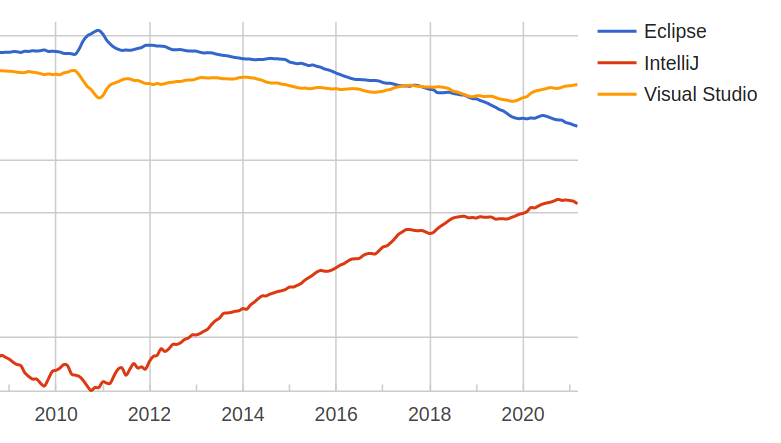
\includegraphics[width=0.8\textwidth]{images/ide-index}
		\label{img:ide-index}
	\end{figure}
	Aus den oben erläuterten Daten und aufgrund der guten Dokumentation für Plugin Entwicklung wird das GuttenBase als ein Intellij Plugin umgesetzt. 
	
	
	\subsection{GuttenBase}
	\label{sec:imp:gb}
	Die Nutzung der GuttenBase Bibliothek wird in folgenden Schritten erklärt.
	%\subsection{Schritt 1: Abhängigkeiten}
	%Um GuttenBase verwenden zu können, soll werden folgende Informationen benötigt:
	%\begin{itemize}
	%	\item groupId: de.akquinet.jbosscc.guttenbase
	%	\item artifactId: GuttenBase
	%	\item version: 2.0.0
	%\end{itemize}
	%Außerdem 
	\paragraph*{Schritt 1: Datenbankverbindung erstellen}
	Als erstes sollen Abhängigkeiten zu dem laufenden Projekt hinzugefügt werden. Die für GuttenBase benötigte Informationen sind:
	\begin{itemize}
		\item groupId: de.akquinet.jbosscc.guttenbase
		\item artifactId: GuttenBase
		\item version: 2.0.0
	\end{itemize}
	Zusätzlich sollen die Treiber-Klassen der Quell- und Ziel-DBMS hinzugefügt werden.\\
	Zunächst sollen die ConnectionInfo Klassen fürerstellt werden. Diese beschreiben die Quell- und Ziel-Datenbanken und enthalten die für eine JDBC (Java Database Connectivity) Verbindung erforderlichen Attribute.\\
	\begin{figure}[H]
		\centering
		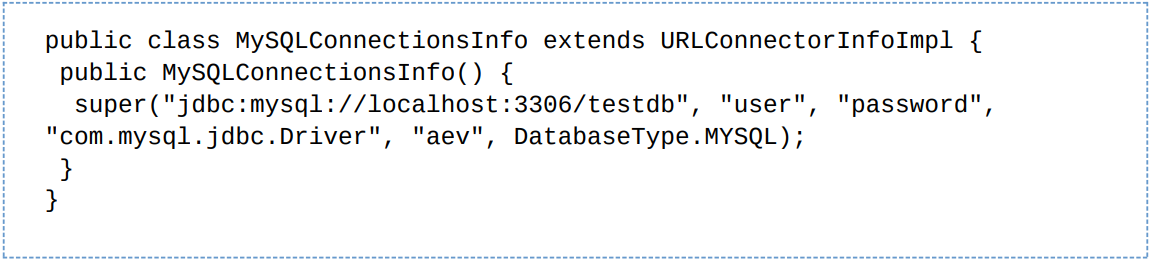
\includegraphics[width=0.8\textwidth]{images/gb/conInfo}
		\caption{ConnectionInfo konfigurieren}
		\label{img:gb/conInfo}
	\end{figure}
	
	Im nachhinein wird das Connector Repository konfiguriert werden. Dies enthält alle Konnektoren, die in der Datenbank Migration beteiligt sind. \\
	\begin{figure}[H]
		\centering
		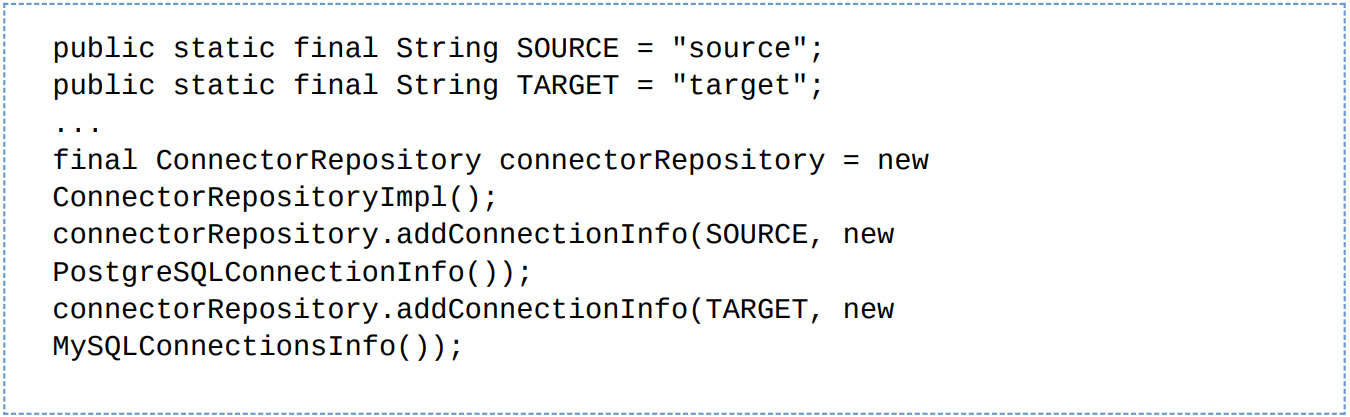
\includegraphics[width=0.8\textwidth]{images/gb/repo}
		\caption{Connector Repository konfigurieren}
		\label{img:gb/repo}
	\end{figure}
	
	\paragraph*{Schritt 2: Hinweise hinzufügen}
	Meistens werden Konfigurationshinweise (hints) benötigt, um die Migration zu individualisieren. In der Dokumentation von GuttenBase\footnote{Getting Started with GuttenBase (2018, 04.01) \\ \url{https://github.com/akquinet/GuttenBase/blob/master/Getting\%20Started\%20with\%20GuttenBase.pdf}} befindet sich eine Liste aller unterstützen Konfigurationshinweise. \\
	Als Beispiel wird der Konfigurationshinweis ColumnMapperHint in der Abbildung dargestellt.
	\begin{figure}[H]
		\centering
		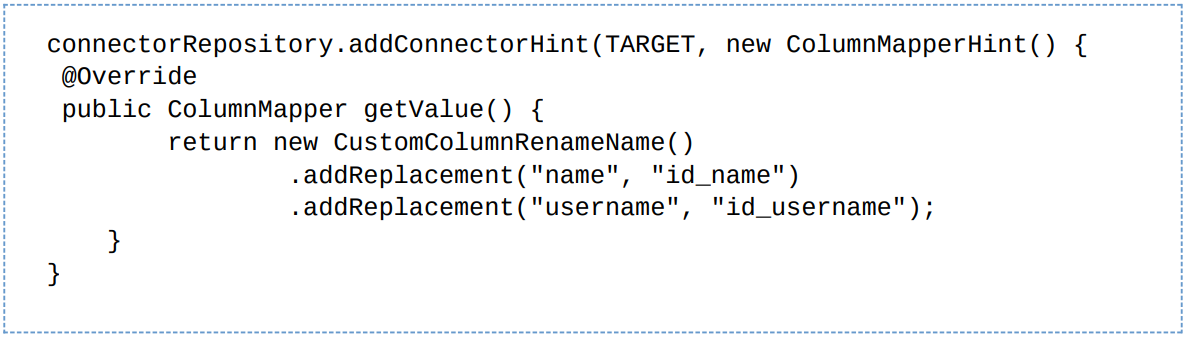
\includegraphics[width=0.8\textwidth]{images/gb/rename}
		\caption{ColumnMapperHint hinzufügen}
		\label{img:gb/rename}
	\end{figure}
	
	
	\paragraph*{Schritt 3: Datenbank Migration durchführen}
	Anschließend kann die Migration mit den eventuell hinzugefügten Hinweisen durchgeführt werden. Dies passiert wie folgt:
	\begin{itemize}
		\item Das Datenbank Schema wird von der Quell-Datenbank in die Ziel-Datenbank kopiert. Dabei werden möglichst viele Unterschiede in Datentypdarstellung standardmäßig berücksichtigt.
		\item Die Kompatibilität von den Schemata wird geprüft. Hierbei wird nach gleichen Tabellen bzw Spalten gesucht.
		\item Falls es keine Fehler beim Prüfen gibt, werden die Daten dann kopiert.
	\end{itemize}
	\begin{figure}[H]
		\centering
		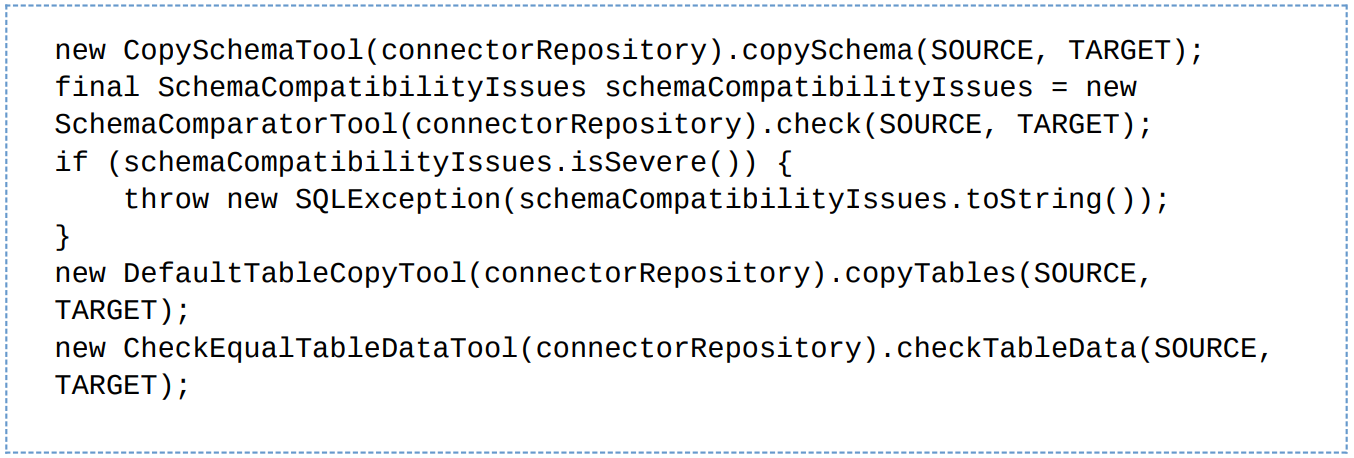
\includegraphics[width=0.8\textwidth]{images/gb/copy}
		\caption{Datenbank Migration durchführen}
		\label{img:gb/copy}
	\end{figure}
	
	
	
	\subsection{IntelliJ Platform}
	Für die erfolgreiche IntelliJ Plugin Entwicklung muss auf mehrere Aspekte geachtet werden wie die Projektstruktur und die häufig verwendeten Komponenten.\\
	Die Plugin Entwicklung erfolgt in der IntelliJ IDE selbst. Deswegen kann das Plugin entweder in Java, Kotlin, Groovy oder Scala geschrieben werden.\\
	Der von Jetbrains empfohlene Weg für das Erstellen eines neuen Plugins ist das Gradle Projekt. Dabei muss die Option IntelliJ Platform Plugin ausgewählt werden, damit die Plugin Abhängigkeiten sowie die Basis-IDE automatisch konfiguriert werden. Zusätzlich muss die Datei plugin.xml entsprechend des zu entwickelnden Plugins angepasst werden. Diese enthält wichtige Informationen, die in den folgenden Tags (Auszeichnungen) erklärt werden:
	\begin{itemize}
		\item \textbf{<name>} \\
		Der Name des Plugins. Er soll kurz und beschreibend sein.
		\item \textbf{<id>} \\
		Eine eindeutige Bezeichnung des Plugins. Diese kann nicht während der Entwicklung geändert werden.
		\item \textbf{<description>} \\
		Eine Kurze Beschreibung des Plugins.
		\item \textbf{<change-notes>} \\
		Eine Beschrei Beschreibung der Änderungen in der neusten Version des Plugins.
		\item \textbf{<version>} \\
		Die aktuelle Plugin Version.
		\item \textbf{<vendor>} \\
		Der Anbieter des Plugins. Hier kann zusätzlich eine Email Adresse angegeben werden.
		\item \textbf{<depends>} \\
		Abhängigkeiten zu Plugins oder Modulen.
		\item \textbf{<idea-version>} \\
		Die minimale und maximale Version der IDE, mit der das Plugin kompatibel ist.
		\item \textbf{<actions>} \\
		Definiert wie die Funktionalität des Plugins aufgerufen wird. Dies wird im folgenden Abschnitt behandelt.
		\item \textbf{<extensionPoints>} \\
		Die vom Plugin definierte Erweiterungspunkte. Diese können erlauben anderen Plugin-Entwicklern, auf bestimmte Daten zuzugreifen. 
		\item \textbf{<extensions>} \\
		Erweiterungspunkte, die von IntelliJ-Platform bzw. von anderen Plugins definiert sind und von dem zu entwickelnden Plugin verwendet werden.
	\end{itemize}
	\subsubsection*{Action-System}
	Die am häufigsten verwendete Methode, um die Plugin Funktionalität aufzurufen, ist die Nutzung der sogenannten Actions vom Action-System der IntelliJ-Platform.\\ \\
	Eine Aktion kann über ein Menüpunkt (menu item) oder einen Eintrag in der Symbolleiste ausgelöst werden. Dazu muss ein Eintrag in dem Actions Tag der plugin.xml Datei erfolgen. Dabei muss jede Action mindestens eine Id, eine Klasse und einen beschreibenden Text haben. I.d.R werden Menüpunkte nach Funktionaliät gruppiert. Um die Implementierte Action zu einer bestimmten Gruppe hinzufügen zu können, muss der Tag \textbf{<add-to-group>} verwendet werden.\\ \\
	Die Action Klasse muss von der AnAction Klasse abgeleitet werden und die actionPerformed() Methode überschreiben. Diese wird nach dem Klick auf das entsprechende Menupunk bzw. Symbolleiste aufgerufen.
	%\subsubsection{Swing}
	%TODO TEST
	%\subsubsection{IntelliJ Plugin Entwicklung}

\section{PlugIn Implementierung}
\subsection{Funktion: Liste der vorhandenen Migrationsoperationen}

	Um die Funktionalität des GuttenBase Plugins einfach und intuitiv für IntelliJ Nutzer zur Verfügung zu stellen, wurden Menüpunkte zum Database Plugin hinzugefügt. Diese wurden gemäß dem Grundsatz der Unterscheidbarkeit plaziert. Somit kann die Übersicht der Migrationsoperationen nach dem Klick auf \glqq Show Migration Actions\grqq geöffnet werden. Dies wird in der Abbildung \ref{img:creategbaction} dargestellt. Diese enthält standardmäßig nur zwei Migrationsoperationen (Tabellen bzw. Spalten Ausschließen).\\ 
	\begin{figure}[h]
		\centering
		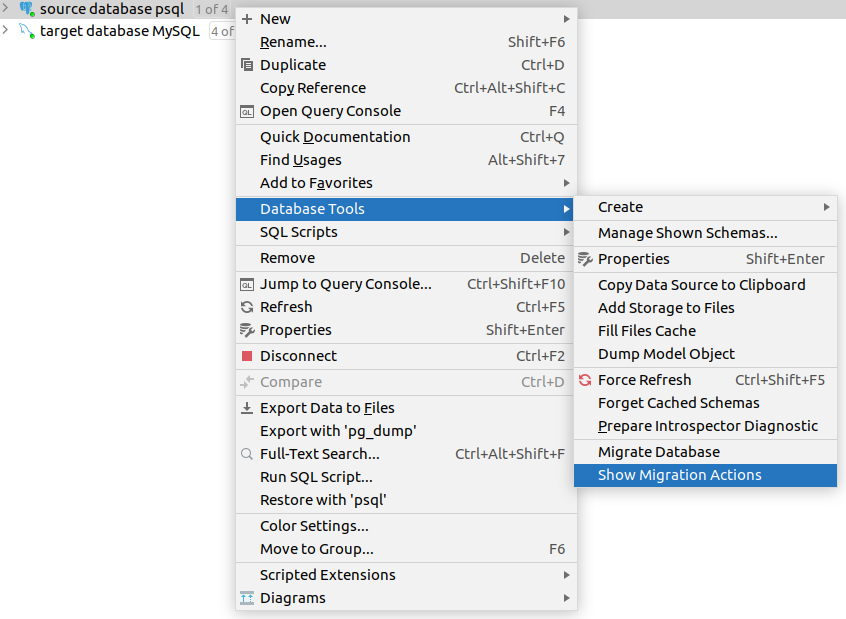
\includegraphics[width=0.7\textwidth]{images/ui/dbactions}
		\caption{Übersicht der Migrationsoperationen öffnen}
		\label{img:dbactions}
	\end{figure}
	%\begin{figure}[h]
	%	\centering
	%	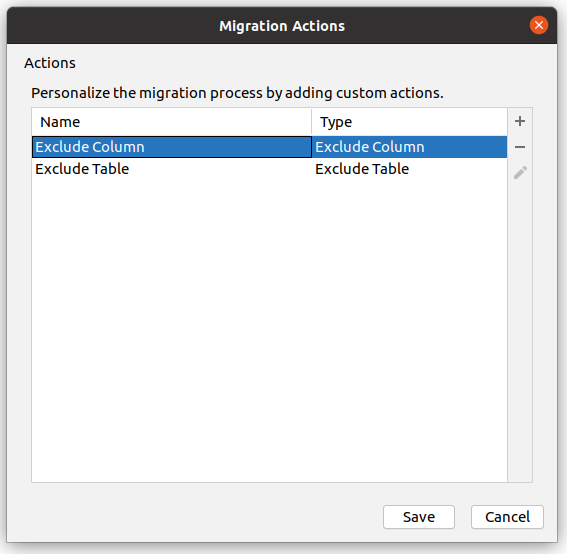
\includegraphics[width=0.5\textwidth]{images/ui/gbactions}
	%	\caption{Übersicht der Migrationsoperationen}
	%	\label{img:gbactions}
	%\end{figure}
	\begin{figure}[H]
		\centering
		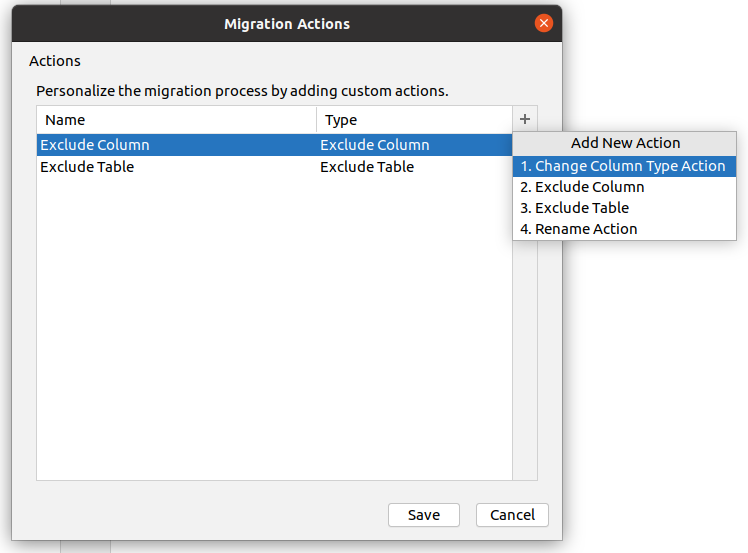
\includegraphics[width=0.7\textwidth]{images/ui/creategbaction}
		\caption{Übersicht der Migrationsoperationen}
		\label{img:creategbaction}
	\end{figure}

\subsection{Funktion: Hinzufügen einer neuen Migrationsoperation}
	
	Bei der Übersicht in der Abbildung \ref{img:creategbaction} kann der Benutzer verschiedene Migrationsoperationen erstellen, wenn diese nicht bereits existieren. In diesem Szenario wird nur das Hinzufügen von der Migrationsoperation Umbenennen (Rename Action) dargestellt.\\
	Nach dem Klick auf das entsprechende Button wird ein Dialog angezeigt, um die erforderliche Informationen einzugeben. Dabei wird der Name der Migrationsoperation festgelegt. Außerdem der Quell-Name durch einen regulären Ausdruck definiert. Anschließend  wird die der Zeil-Name festgelegt. \\
	Die in der Abbildung \ref{img:createRename} angezeigte Migrationsoperation gilt für alle Datenbankelemente, deren Name die Zeichenkette \glqq table\grqq enthält. Wenn diese an einem entsprechenden Datenbankelement angewendet wird, wird das Suffix \glqq \_Test\grqq \, hinten hinzugefügt.
	\begin{figure}[h]
		\centering
		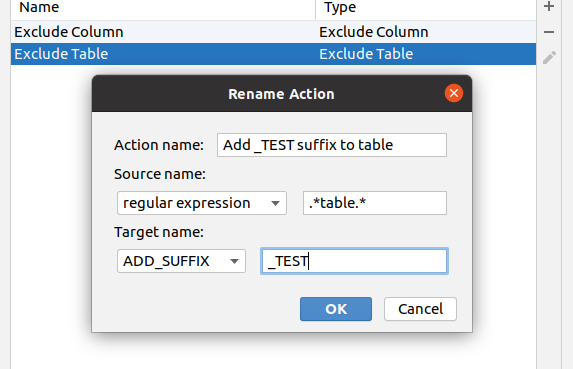
\includegraphics[width=0.5\textwidth]{images/ui/createRename}
		\caption{Migrationsoperation Umbenennen erstellen}
		\label{img:createRename}
	\end{figure}
	%Der reguläre Ausdruck \textbf{.*table.*} bedeutet im dargestellten Beispiel, dass die erstellte 
	Anschließend lässt sich die neu hinzugefügte Migrationsoperation durch das Klick auf das \glqq Save\grqq \, Button speichern (siehe Abbildung \ref{img:creategbaction}). Dabei werden alle Migrationsoperationen nach JSON konvertiert und in einer externen Datei gespeichert. Dafür ist die Klasse GsonHelper verantwortlich (siehe Abbildung \ref{img:gson}).
	\begin{figure}[h]
		\centering
		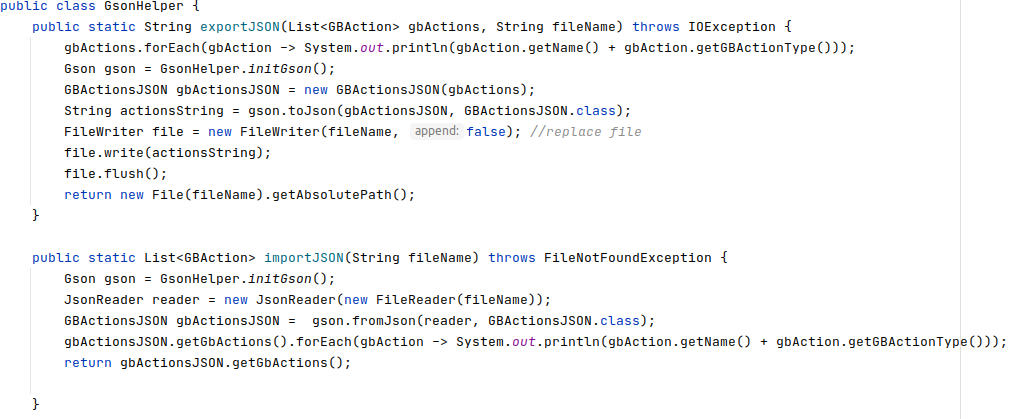
\includegraphics[width=0.9\textwidth]{images/ui/gson}
		\caption{Migrationsoperationen exportieren und importieren}
		\label{img:gson}
	\end{figure}
	
\subsection{Funktion: Verbindungerstellung}
		
	Wenn die Quell- und Ziel-Datenbank im Database Plugin eingerichtet sind, kann das Aktionsmenü nach Rechtsklick auf die Quell-Datenbank aktiviert werden. Wie in der Abbildung \ref{img:dbactions} angezeigt, kann der Benutzer auf das Button \glqq Migrate Database\grqq \, klicken um die Übersicht der Datenbank Migration zu öffnen (siehe Abbildung \ref{img:ui:generalView}). Dabei wird die Quell-Datenbank anhand der selektierten Datenbank automatisch selektiert. Außerdem muss das zu migrierende Schema der Quell-Datenbank sowie das Ziel-Schema ausgewählt werden. Zusätzlich müssen die Zugangsdaten jeder Datenbank angegeben werden, um die Datenbanken zu verbinden.
	\begin{figure}[h]
		\centering
		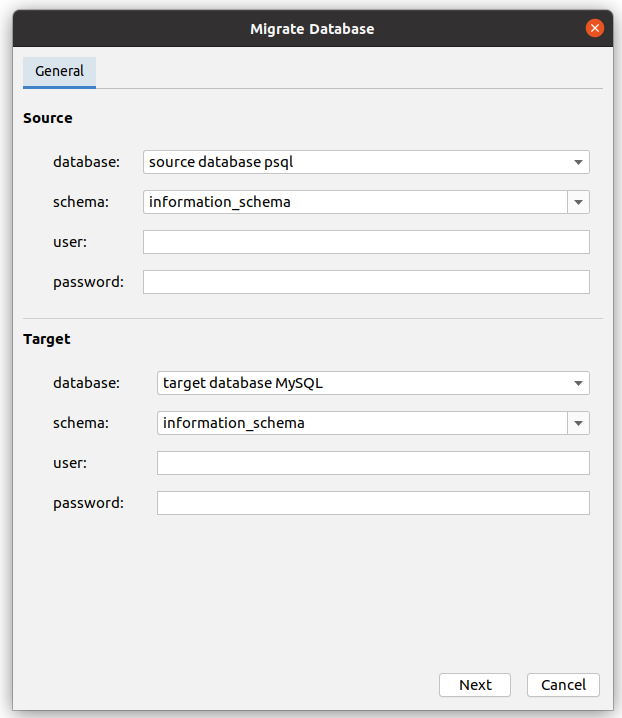
\includegraphics[width=0.5\textwidth]{images/ui/generalView}
		\caption{Allgemeine Übersicht der Datenbank Migration (generalView)}
		\label{img:ui:generalView}
	\end{figure}
	Nach dem Klick auf das \glqq Next\grqq \, Button, werden die Angaben erst geprüft. Wenn diese fehlerhaft sind, dann wird eine entsprechende Fehlermeldung ausgegeben. Ansonsten wird das ConnectorRepository (siehe \ref{sec:imp:gb}) anhand der angegebenen Informationen erstellt und anschließend die nächste Übersicht (overview) angezeigt.
	
\subsection{Funktion: Konfiguration}
	
	Bei der Konfigurationsüberischt (siehe Abbildung \ref{img:ui:overviewSingleAdd}) werden alle Elemente der Quell-Datenank anzgezeigt. Hierbei wird Einzel- sowie Mehrfachauswahl ermöglicht. \\
	\begin{figure}[h]
		\centering
		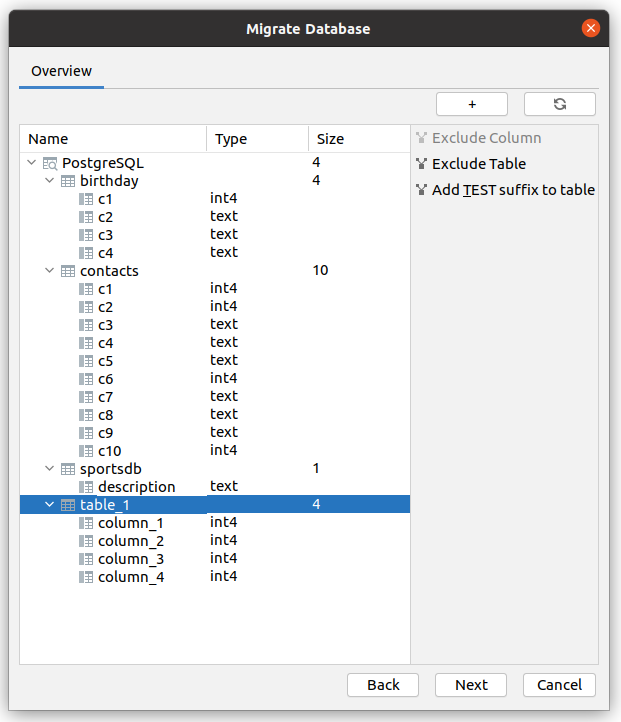
\includegraphics[width=0.5\textwidth]{images/ui/overviewSingleAdd}
		\caption{Konfigurationsübersicht (overview)}
		\label{img:ui:overviewSingleAdd}
	\end{figure}
	Außerdem werden alle Migrationsoperationen mithilfe der \textbf{GsonHelper} Klasse geladen werden. Diese werden abhängig von den selektierten Elementen unterschiedlich dargestellt. Wenn eine Migrationsoperation (GBAction) zu den ausgewählten Elementen passt, wird diese klickbar angezeigt, ansonsten wird diese deaktiviert und ausgegraut dargestellt. Dabei spielt die \textbf{matches} Methode der \textbf{GBAction} Klasse eine entscheidende Rolle. Diese wird entsprechend des Typen der Migrationsoperation. Für das Umbenennen wird z. B. geprüft, ob der gespeicherte reguläre Ausdruck zum Namen der selektierten Elemente passt (siehe Abbildung \ref{img:ui:matches}).
	
	\begin{figure}[h]
		\centering
		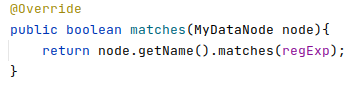
\includegraphics[width=0.5\textwidth]{images/ui/matches}
		\caption{matches Methode der Migrationsoperation Umbenennen}
		\label{img:ui:matches}
	\end{figure}
	Bei jedem Hinzufügen wird die entsprechende Migrationsoperation zu der Liste aller Operationen hinzugefügt. Dabei wird eine neue Instanz erzeugt, die die benötigten Informationen des entsprechenden Datenbankelementes enthält (siehe Abbildung \ref{img:ui:overviewAddRenameSrc}).
	%overviewAddRenameSrc
	\begin{figure}[H]
		\centering
		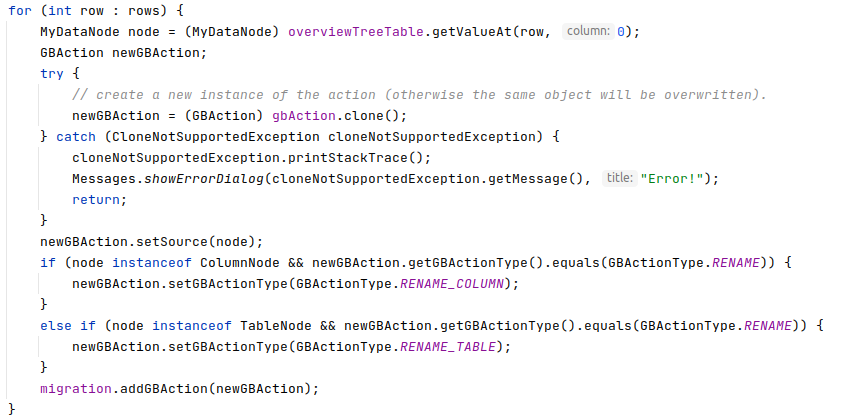
\includegraphics[width=0.9\textwidth]{images/ui/overviewAddRenameSrc}
		\caption{das Hinzufügen von der Migrationsoperation Umbenennen}
		\label{img:ui:overviewAddRenameSrc}
	\end{figure}
\subsection{Funktion: Migrationsdurchführung}
	
	Nach dem Klick auf das \glqq Next\grqq \, Button, erhält der Benutzer eine Übersicht von allen hinzugefügten Migrationsoperationen (siehe Abbildung \ref{img:ui:resultView}). Diese können nach Bedarf gelöscht werden.\\
	\begin{figure}[H]
		\centering
		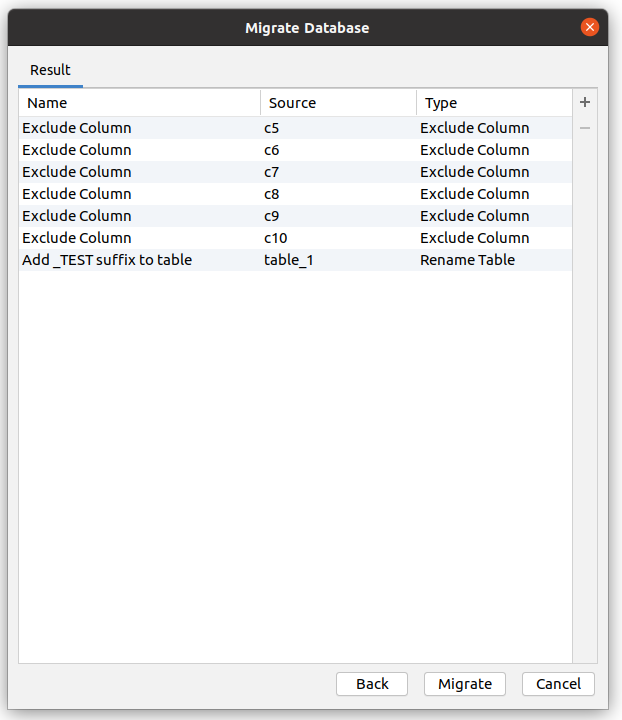
\includegraphics[width=0.5\textwidth]{images/ui/resultView}
		\caption{Ergebnisübersicht}
		\label{img:ui:resultView}
	\end{figure}
	Nach dem Klick auf das \glqq Migrate\, Button, wird die Fortschrittsübersicht angezeigt (siehe Abbildung \ref{img:ui:progressView}). Diese veranschaulicht den Migrationsprozess, welcher in einem neuen Thread ausgeführt wird. Bei der Migration werden die Mapper Klassen sowie die GuttenBase Connectors (siehe Abschnitt \ref{sec:imp:gb}) entsprechend der hinzugefügten Migrationsoperationen zum ConnectorRepository hinzugefügt. Danach werden die Daten von der Quell-Datenbank zur Zie-Datenbank kopiert (siehe Abbildung \ref{img:ui:connectors} bzw. Abbildung \ref{img:ui:run}). \\
	\begin{figure}[H]
		\centering
		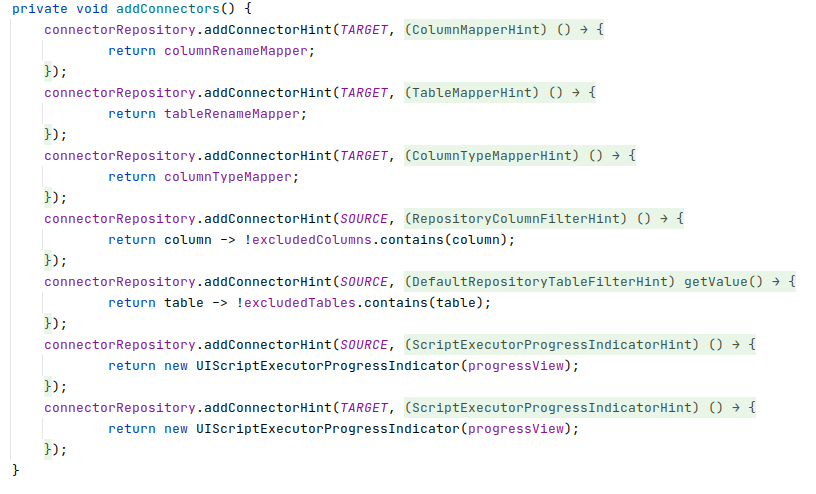
\includegraphics[width=0.9\textwidth]{images/ui/connectors}
		\caption{ConnectorHints hinzufügen}
		\label{img:ui:connectors}
	\end{figure}
	\begin{figure}[H]
		\centering
		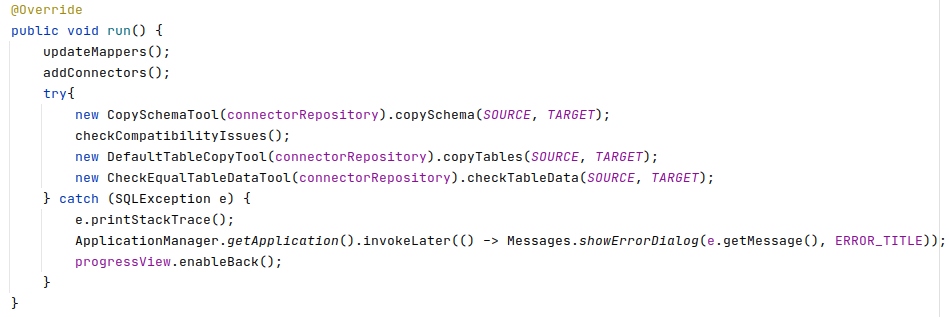
\includegraphics[width=0.9\textwidth]{images/ui/run}
		\caption{Migration durchführen (MapperHelper Klasse)}
		\label{img:ui:run}
	\end{figure}
	
	Falls ein Fehler bei der Migration auftritt, wird eine entsprechende Fehlermeldung angezeigt und das \glqq Back\grqq \, aktiviert, um Änderungen durchzuführen und die Migration nochmal zu starten. Der Benutzer bekommt außerdem einen Hinweis, Falls die Migration erfolgreich abgeschlossen ist.
	\begin{figure}[H]
		\centering
		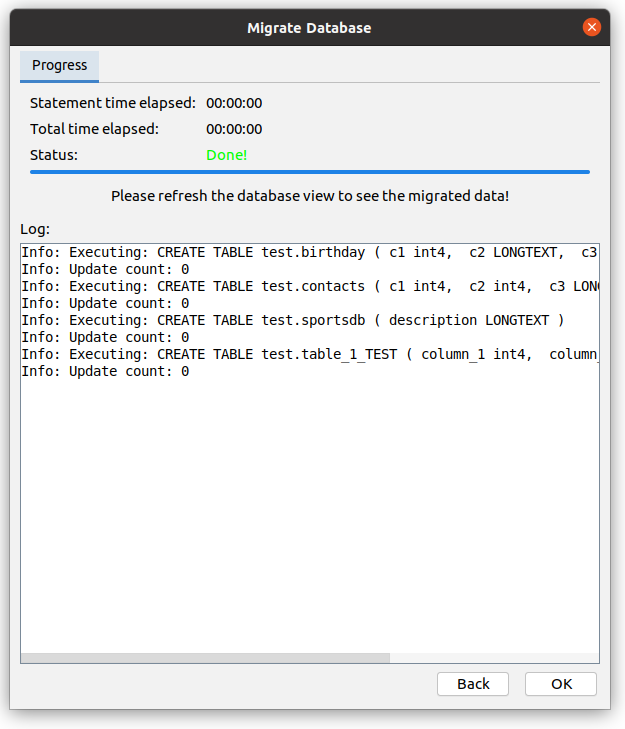
\includegraphics[width=0.5\textwidth]{images/ui/progressView}
		\caption{Fortschrittsübersicht}
		\label{img:ui:progressView}
	\end{figure}